\documentclass{beamer}
\usepackage[utf8]{inputenc}
\usetheme[background=dark,titleformat = smallcaps , block = fill,numbering = fraction, progressbar = 
frametitle , titleformat title= smallcaps]{metropolis}           % Use metropolis theme


\definecolor{orangeBar}{HTML}{FF3600}
\setbeamercolor{progress bar}{fg=orangeBar}

\usepackage{multimedia}
\usepackage{animate}
\usepackage {extarrows}
\usepackage {tikz}
\usepackage[options ]{algorithm2e}
\usepackage[spanish]{babel}
\usepackage{graphicx}
\usepackage{amssymb}
%\usepackage{amsfonts}

\usepackage{enumerate}
\usepackage{amsmath}
\usepackage{amsthm}
\usepackage{xcolor}
%\usepackage{amsfonts,amssymb,amsthm}

\usepackage{url}
\usepackage{enumerate}
\usepackage{commath}
\usepackage{multicol}
\usepackage{mathtools}
\usepackage{scrextend}
\usepackage{hyperref}
\usepackage{cleveref}
\usepackage{longtable}
\usepackage{bbm}
\usepackage{siunitx}
\usepackage{listings}
\usepackage{xcolor}
\usepackage{subcaption}
\usepackage{epigraph}
\usetikzlibrary{arrows}

\definecolor{codegreen}{rgb}{0,0.6,0}
\definecolor{codegray}{rgb}{0.5,0.5,0.5}
\definecolor{codepurple}{rgb}{0.58,0,0.82}
\definecolor{backcolour}{rgb}{0.95,0.95,0.92}
\definecolor{darkBlue}{HTML}{00000F}
\definecolor{lightBlue}{HTML}{00B7D4}
\definecolor{lightRed}{HTML}{E42525}
\definecolor{lightGreen}{HTML}{9CE425}

\definecolor{green0}{HTML}{B65900}
\definecolor{green1}{HTML}{D77200}
\definecolor{green2}{HTML}{ED8E30}
\definecolor{green3}{HTML}{FABE86}

\lstdefinestyle{mystyle}{
    backgroundcolor=\color{darkBlue},   
	commentstyle=\color{lightGreen},
	keywordstyle=\color{lightBlue},
	numberstyle=\tiny\color{codegray},
	stringstyle=\color{lightRed},
	basicstyle=\ttfamily\footnotesize,
	breakatwhitespace=false,         
	breaklines=true,                 
	captionpos=b,                    
	keepspaces=true,                 
	numbers=left,                    
	numbersep=5pt,                  
	showspaces=false,                
	showstringspaces=false,
	showtabs=false,                  
	tabsize=1
}

\lstset{style=mystyle}
\lstset{language=Python}
\lstset{frame=lines}
\lstset{caption={Insert code directly in your document}}
\lstset{label={lst:code_direct}}
\lstset{basicstyle=\footnotesize}


\newcommand{\bb}[1]{\mathbb{#1}}

%\newtheorem{theorem}{Teorema}[section]
%\theoremstyle{plain}
\newtheorem{acknowledgement}[theorem]{Acknowledgement}
%\newtheorem{algorithm}[theorem]{Algorithm}
\newtheorem{axiom}[theorem]{Axiom}
\newtheorem{case}[theorem]{Case}
\newtheorem{claim}{Claim}
\newtheorem{conclution}[theorem]{Conclusión}
\newtheorem{condition}[theorem]{Condition}
\newtheorem{conjecture}[theorem]{Conjecture}
%\newtheorem{corollary}[theorem]{Corolario}
\newtheorem{criterion}[theorem]{Criterion}
\theoremstyle{definition}
%\newtheorem*{df}{Definición}
%\newtheorem{definition}[theorem]{Definición}
%\newtheorem{example}[theorem]{Ejemplo}
\newtheorem{exercise}[theorem]{Exercise}
%\newtheorem{lemma}[theorem]{Lema}
\newtheorem{notation}[theorem]{Notation}
%\newtheorem{problem}[theorem]{Problem}
\newtheorem{proposition}[theorem]{Proposición}
\newtheorem{remark}[theorem]{Nota}
%\newtheorem{solution}[theorem]{Solución}
\newtheorem{summary}[theorem]{Summary}
\numberwithin{equation}{section}

\definecolor{defColor}{HTML}{3ED597}
\newcommand{\marine}[1]{\textcolor{defColor}{#1}}


\definecolor{thColor}{HTML}{FA7E0A}
\newcommand{\orangee}[1]{\textcolor{thColor}{#1}}

\definecolor{rkColor}{HTML}{F72121}
\newcommand{\redd}[1]{\textcolor{rkColor}{#1}}


%---------------emojis--------------------
\newcommand{\smiley}{\tikz[baseline=-0.75ex,black]{
		\draw circle (2mm);
		\node[fill,circle,inner sep=0.5pt] (left eye) at (135:0.8mm) {};
		\node[fill,circle,inner sep=0.5pt] (right eye) at (45:0.8mm) {};
		\draw (-145:0.9mm) arc (-120:-60:1.5mm);
	}
}

\newcommand{\frownie}{\tikz[baseline=-0.75ex,black]{
		\draw circle (2mm);
		\node[fill,circle,inner sep=0.5pt] (left eye) at (135:0.8mm) {};
		\node[fill,circle,inner sep=0.5pt] (right eye) at (45:0.8mm) {};
		\draw (-145:0.9mm) arc (120:60:1.5mm);
	}
}

\newcommand{\neutranie}{\tikz[baseline=-0.75ex,black]{
		\draw circle (2mm);
		\node[fill,circle,inner sep=0.5pt] (left eye) at (135:0.8mm) {};
		\node[fill,circle,inner sep=0.5pt] (right eye) at (45:0.8mm) {};
		\draw (-135:0.9mm) -- (-45:0.9mm);
	}
}




\newtheorem{df}{\marine{Definición}}
\newtheorem{thh}{\orangee{Teorema}}
\newtheorem{pr}{\orangee{Proposición}}
\newtheorem{lm}{\orangee{Lema}}
\newtheorem{crr}{\orangee{Corolario}}
\newtheorem{rr}{\redd{Observación}}
\usepackage{graphicx} 


%\newtheorem{defn}[]{Definición}
%\newenvironment{definition}{\begin{defn}}{\end{defn}}
%\newtheorem{definition}{Definition}[section]
%\newtheorem*{remark}{Remark}
%%%%%%%%
\newcommand{\tit}[1]{\textit{#1}}
\newcommand{\bsym}{\mathbf}
\newcommand{\Mod}[1]{\ (\mathrm{mod}\ #1)}
%\newcommand{\blue}[1]{\textcolor{blue}{#1}}
\newcommand{\red}[1]{\textcolor{red}{#1}}
\renewcommand{\geq}{\geqslant}
\renewcommand{\leq}{\leqslant}
\newcommand{\Rplus}{\mathds{R}_{^{+}}}
\newcommand{\N}{\mathbb{N}}
\newcommand{\Z}{\mathbb{Z}}
\newcommand{\R}{\mathbb{R}}

\newcommand{\C}{\mathbb{C}}
\newcommand{\Q}{\mathbb{Q}}
\newcommand{\ssi}{\longleftrightarrow}
\newcommand{\ent}{\longrightarrow}
\newcommand{\Qp}{\mathbb{Q}_p}  
\newcommand{\Qpn}{\mathbb{Q}_p^n}
\newcommand{\Zpn}{\mathbb{Z}_p^n}
\newcommand{\Zp}{\mathbb{Z}_p}
\newcommand{\Zd}{\mathbb{Z}_2}
%\newcommand{\abs}[1]{\left\vert #1 \right\vert}
%\newcommand{\norm}[1]{\|#1\|}
\newcommand{\pnorm}[1]{\|#1\|_p}
\newcommand{\maxx}[1]{\text{m\'ax} #1}
\newcommand{\xbar}[1]{\hskip 1.4pt\overline{\hskip-1.2pt #1\hskip -.6pt}\hskip 1.2pt}
\newcommand{\rb}{\raisebox{-.35ex}}

\DeclareMathOperator{\s}{\mathbf{S}}
\DeclareMathOperator{\f}{\mathcal{F}}
\DeclareMathOperator{\A}{\mathbb{A}}
\DeclareMathOperator{\dist}{dist} % The distance.
\DeclareMathOperator{\d^n}{\dif^{\,n}}
%\DeclareMathOperator{\d}{\dif}
\DeclareMathOperator{\Real}{Re}
\DeclareMathOperator{\ord}{Ord}
\DeclareMathOperator{\Dom}{Dom}
\DeclareMathOperator{\vol}{vol}
\DeclareMathOperator{\gpn}{\mathit{{GpnN}}}
%%%%%%%%%
%%%%%%%%%%%%%%%%% dashed integrals %%%%%%%%%%%%%%%%%%%%%
\DeclareSymbolFont{eulargesymbols}{U}{zeuex}{m}{n}
\DeclareMathSymbol{\intop}{\mathop}{eulargesymbols}{"52}
\usepackage[toc,page]{appendix}
\renewcommand{\labelitemi}{$\circ$}


\title{Análisis de la infraestructura turística de las principales ciudades del país}
\subtitle{Proyecto final, Estadística Multivariada}
\date{27 de Mayo de 2021}


\author{\bf{Autores: }Edgar Baquero \& Enrique Santibáñez}

\institute{Centro de Investigación en Matemáticas, \\Maestría en Cómputo Estadístico.}
%Facultad de Ciencias\\
%Departamento de Matemáticas}



\usepackage{MnSymbol,wasysym}



\titlegraphic{%
	\begin{picture}(0,0)
	\put(190,-190){\makebox(0,0)[rt]{
\includegraphics[width=2cm]{logo}}}
    \end{picture}
}

\usepackage[backend=biber, style=apa, natbib = true]{biblatex}
\bibliography{biblio.bib}

\title{Comparaciones Múltiples Y False Discovery Rate y su relación con Ciencia de Datos}
\subtitle{Maestría en Cómputo Estadístico}
\date{\today}
\author{\bf{Autores: } Enrique Santibáñez \& Edgar Baquero}
\institute{Centro de Investigacón en Matemáticas, A.C.}
\usepackage{MnSymbol,wasysym}

%logo U
\titlegraphic{%
	\begin{picture}(0,0)
	\put(180,-190){\makebox(0,0)[rt]{
\includegraphics[width=2cm]{logo_U_Mty.png}}}
	\end{picture}
}

\begin{document}
  \maketitle




\begin{frame}{Contenido}
	\tableofcontents
\end{frame}
%------parte Edgar: MCP-----------------------
\section{Introducción}
\begin{frame}{Introducción}
    Papel de la inferencia estadística
    \begin{itemize}[<+- | alert@+>]
        \item Cuestionarse acerca de parámetros que estimamos.
        \item Lo hacemos a través de \textit{Pruebas de Hipótesis}.
        \item Generalmente queremos comparar más de dos parámetros.
        \item Este proceso se conoce como Comparación Múltiple.
    \end{itemize}
\end{frame}
\section{Aspectos preliminares}
\begin{frame}{Pruebas de hipótesis simples}
    \begin{df}
        Se conoce como hipótesis \textit{simple}, a una prueba en la que interviene sólo una única hipótesis nula $H_0$ y su complemento, la hipótesis alternativa $H_1$.
    \end{df}
    \begin{example}[Un quiz chévere...]
        \begin{itemize}[<+- | alert@+>]
        \item \textit{Fat Tony} va a ser juzgado como mafioso, y el Juez \textit{Roy Snyder} lo hará:
            \item 
\includegraphics[scale = 0.15]{cheve.png}
            \item 
\includegraphics[scale = 0.12]{Acusado.png}\quad \quad  
\includegraphics[scale = 0.15]{Juez.png}
        \end{itemize}
    \end{example}
\end{frame}

\begin{frame}{Pruebas de hipótesis simples}
    \begin{example}[Juicio oral - Continuación]
        \textit{Roy Snyder} plantea:
        \begin{itemize}
            \item $H_0$ : \textit{Fat Tony} es inocente.
            \item $H_1$ : \textit{Fat Tony} es culpable.
        \end{itemize}
        Los posibles resultados del juicio pueden mostrarse en la siguiente tabla:
        \begin{center}
            \scalebox{0.8}{ 
        	\begin{tabular}{ | m{4.3cm} | m{3.3cm}| m{3.3cm} | } 
        		\hline
        		& $H_0$ Cierta (inocencia) & $H_0$ Falsa (Culpable)\\ 
        		\hline
        		$H_0$ rechazada (Condenado) & Error tipo I & Decisión correcta\\ 
        		\hline
        		$H_0$ no rechazada (Libre)  & Decisión correcta& Error tipo II\\ 
        		\hline
        	\end{tabular}
        	}
        \end{center}
    \end{example}
\end{frame}




\begin{frame}{Pruebas de hipótesis simples}
    \begin{rr}
        En el anterior ejemplo, pareciera que no tuviéramos relación entre el error tipo I y el error tipo II. Aún así, es posible probar que:
        \begin{itemize}
            \item $P(\textit{error tipo I })\to0\quad \Longrightarrow \quad P(\textit{error tipo II} )\to 1$
            \item $P(\textit{error tipo II})\to0\quad \Longrightarrow \quad P(\textit{error tipo I } )\to 1$
        \end{itemize}
    \end{rr}
    \begin{itemize}[<+- | alert@+>]
        \item Casi siempre damos prioridad a disminuir el error tipo I.
        \item En los casos donde se requiere controlar el error tipo II, trabajamos con \textit{pruebas uniformemente más potentes}.
        \item Dado que el error tipo I quiere llevarse a 0, establecemos una cota superior para la cual este puede ser encontrado. Dicha cota se conoce como \textit{nivel de significancia} y se denota con la letra $\alpha$
        
    \end{itemize}
\end{frame}

\begin{frame}{Pruebas de hipótesis simples - Definiciones}
    
    Una vez establecida la filosofía básica de una prueba de hipótesis, planteamos algunos conceptos:
    \begin{df}
    \begin{itemize}
        \item \textbf{Hipótesis de trabajo:} La aseveración acerca del espacio parametral $\Theta$ que nos interesa probar,
        junto con su complemento o hipótesis alternativa. Usualmente es denotado de la siguiente forma:
        $$H_0:\theta\in\Theta_0; \quad H_1: \theta\in\Theta_1,$$
        donde $\{\Theta_0,\Theta_1\}$ es una partición de $\Theta$, el espacio de parámetros.
    \end{itemize}
    \end{df}
\end{frame}

\begin{frame}{Pruebas de hipótesis simples - Definiciones}
    \begin{df}[Continuación]
    \begin{itemize}
        \item \textbf{Estadístico de prueba:} Valor calculado en función de la muestra observada, denotado por $T$.
        \item {Región de Rechazo ($C$): } Conjunto de valores que puede tomar el estadístico de prueba $T$, para los cuales se rechaza $H_0$.
        \item {Potencia: } robabilidad de no cometer error de tipo II. En el caso de una hipótesis que plantee igualdad:
        \begin{equation}
        	\beta(\theta^*)=P(T\in C|\theta=\theta^*)\label{pot}
        \end{equation}
    \end{itemize}
    \end{df}
\end{frame}

\begin{frame}{Pruebas de hipótesis simples - Definiciones}
    \begin{df}[Continuación]
    \begin{itemize}
        \item Nivel de significancia ($\alpha$): puede ser definido en términos de (\ref{pot}):
        \begin{equation}
        	\alpha\leq\sup_{\theta\in\Theta_0} \beta(\theta).
        \end{equation}
        \item \textbf{$p$-valor: } probabilidad, asumiendo la hipótesis nula como cierta, de haber observado un valor del estadístico de prueba al menos tan extremo como el que se observó:
        \begin{equation*}
        	p=P(T>T_{obs}|\theta\in\Theta_0).
        \end{equation*}
    \end{itemize}
    \end{df}
\end{frame}

\begin{frame}{Pruebas de hipótesis simples - Resumen}
En resumen, realizar una prueba de hipótesis consiste en:
\begin{enumerate}[<+- | alert@+>][I]
    \item Plantear la hipótesis nula y la hipótesis alternativa.
	\item Seleccionar un nivel de significancia $\alpha$. El umbral probabilı́stico bajo el cual la hipótesis será rechazada.
	\item Elegir la estadística de prueba adecuada $T$.
	\item Encontrar la distribución de $T$ bajo la hipótesis nula.
	\item Calcular la región crítica o región de rechazo $C$.
	\item Encontrar el valor observado del estadístico de prueba $T_{obs}$ de la muestra o, alternativamente, el $p$-valor.
	\item Decidir si rechazar o no $H_0$ con base en la región $C$ especificada en el paso (VI), o, alternativamente, rechazar $H_0$ si el $p$-valor obtenido pequeño.
\end{enumerate}
\end{frame}

\section{Comparaciones Múltiples}

\begin{frame}{Comparaciones Múltiples - Procedimiento}
\begin{itemize}[<+- | alert@+>]
    \item Es posible juzgar acerca de un determinado número $m>1$ de hipótesis nulas $H_{01},\dots,H_{0m}$.
	\item Es pertinente la realización de un procedimiento que nos permita evaluar la veracidad de una hipótesis general.
	\item \textit{Dutoit} et al (2003), estandarizó el procedimiento
	\item Elegir y calcular un estadístico de prueba $T_j$ para cada hipótesis individual $j$, con $j=1,\dots,m$
	\item Aplicar un procedimiento de prueba de hipótesis múltiple para determinar cuáles hipótesis se han
	de rechazar de manera que se controle de alguna forma específica el error tipo I.
\end{itemize}
\end{frame}


\subsection{Sobre la extensión del caso simple}
\begin{frame}{Sobre la extensión del caso simple}
\begin{itemize}[<+- | alert@+>]
    \item Una prueba de manea simultánea al conjunto de hipótesis $\{H_{01},\dots,H_{0m}\}$ no es equivalente a realizar $m$ pruebas individuales.
    \item Primero, se necesitarían ${m\choose2}=\frac{m(m-1)}{2}$ comparaciones individuales.
    \item Segundo, con mayor relevacia, por independencia entre las hipótesis.
    \item Esto es, el rechazo de $H_{0i}$ podrı́a influir (positiva o negativamente) en las posibilidades del rechazo de $H_{0j}$
\end{itemize}
\end{frame}


\begin{frame}{Sobre la extensión del caso simple}
\begin{example}[Lanzamiento de monedas - parte 1]
    \begin{itemize}[<+- | alert@+>]
        \item Queremos probar si una moneda es equilibrada.
        \item 9 de 10 lanzamientos son cara.
        \item La probabilidad de que se observe un resultado al menos tan extremo como ese, sería de $(10 + 1)(1/2)^{10} = 0.0107$.
        \item Concluimos que la moneda no es justa.
    \end{itemize}
\end{example}
\end{frame}


\begin{frame}{Sobre la extensión del caso simple}
\begin{example}[Lanzamiento de monedas - parte 2]
    \begin{itemize}[<+- | alert@+>]
        \item Repitamos el experimento con 100 monedas.
        \item Esperaríamos que fuera igual o más raro, al lanzar una moneda equilibrado, observar 9 caras en 10 lanzamientos.
        \item ¡Pues no!
        \item De hecho la probabilidad de que en 100 repeticiones al menos una moneda sea equilibrada está dada por $1 - (1 - 0,0107)^{100}= 0.6604$
        \item ¡Sería un error aplicar el razonamiento anterior para probar que las 100 monedas son equilibradas!
    \end{itemize}
\end{example}
\end{frame}

\begin{frame}{Sobre la extensión del caso simple}
\begin{rr}
\begin{itemize}
    \item El anterior ejemplo, nos muestra la delicadeza de la multiplicidad.
    \item La noción de error se complica de manera creciente.
    \item  Si una prueba simple se hace a un $5\%$ de confianza, afirmamos que existe un $5\%$ de probabilidad de que la hipótesis nula sea rechazada incorrectamente.
    \item Si se realizan $m = 100$ pruebas de hipótesis simultáneamente, donde todas son ciertas, el número esperado de rechazos incorrectos es 5
    \item Si las pruebas son independientes, la probabilidad de rechazar al menos una hipótesis incorrectamente es de $1 - (1-0,05)^{100} =0,994$!!!
\end{itemize}
\end{rr}
\end{frame}


\subsection{Sobre el error}
\begin{frame}{Tabla de comparaciones múltiples}
\scalebox{0.8}{ 
\begin{center}
\begin{tabular}{|l|l|l|l|}
	\hline & Hipótesis No Rechazadas & Hipótesis Rechazadas & Total \\
	\hline Hipótesis Verdaderas & $U$ & $V$ & $m_{0}$ \\
	Hipótesis Falsas & $K$ & $S$ & $m_{1}$ \\
	\hline & $m-R$ & $R$ & $M$ \\
	\hline
\end{tabular}	
\end{center}
}
\begin{itemize}
	\item $m$ es el total de hipótesis realizadas.
	\item $m_0$ es el número de hipótesis nulas verdaderas.
	\item $m-m_0$ es el número de verdaderas hipótesis alternativas.
	\item $V$ es el número de falsos positivos (error tipo I) (también conocido como \textit{falso descubrimiento}).
	\item $S$ es el número de verdaderos positivos (conocido como \textit{descubrimiento verdadero}).
	\item $K$ es el número de falsos negativos (error tipo II).
	\item $U$ es el número de verdaderos negativos.
	\item $R=V+S$ es el número de hipótesis nulas rechazadas (conocido como \textit{descubrimientos})
\end{itemize}
\end{frame}




\begin{frame}{Sobre los errores}
Nos encontramos con la necesidad de controlar el error tipo I en el caso múltiple. Para esto, introducimos 3 nociones de error:
\begin{itemize} [<+- | alert@+>]
	\item \textbf{Tasa de Error por Comparación (PCER)}: Consiste de el valor esperado de errores de tipo I dividido entre el número total de hipótesis:
$$
\mathrm{PCER}=\frac{\mathrm{E}(V) }{m}
$$
    \item \textbf{Tasa de Error Global (FWER)}: Es la probabilidad de cometer uno o más errores de tipo I:
$$
\mathrm{FWER}=P(V \geq 1) \Longleftrightarrow \mathrm{FWER}=P(V>0)=1-P(V=0)
$$
\item \textbf{Tasa de Falsos Descubrimientos (FDR)}. se define como el valor esperado de $Q$:
$$
Q=\left\{\begin{array}{ll}
	V/R, & R>0 \\
	0, & R=0
\end{array}\right.
$$
\end{itemize}
\end{frame}

\section{Controlando el FWER}

\begin{frame}{Control del FWER}
\begin{df}
Si suponemos que FWER$\leq\alpha$, decimos que 	la probabilidad de cometer un error tipo I está \textit{controlada} por un nivel $\alpha$. Adicionalmente:
\begin{itemize}
    \item Un proceso controla el FWER \textit{débilmente}, si el control del FWER a un nivel $\alpha$, es garantizado sólo cuando todas las hipótesis  nulas son ciertas.
    \item Un procedimiento controla \textit{fuertemente}, si el control del FWER a un nivel $\alpha$ independientemente de la configuración de hipótesis falsas o verdaderas.
\end{itemize}
\end{df}
\end{frame}

\begin{frame}{Procedimientos de Control del FWER - Bonferroni}
\begin{itemize}[<+- | alert@+>]
    \item Sea $\{H_{01},\dots,H_{0m}\}$ una familia de hipótesis.
    \item Sea $p_i$ el $p$-valor correspondiente a la hipótesis $H_{0i}$.
    \item Procedemos a rechazar la hipótesis $H_{0i}$, si $p_i\leq\frac{\alpha}{m}$
    \item El control puede ser probado a través de la \textit{desigualdad de Boole:}
$$\mathrm{FWER}=P\left\{\bigcup_{i=1}^{m_{0}}\left(p_{i} \leq \frac{\alpha}{m}\right)\right\} \leq \sum_{i=1}^{m_{0}}\left\{P\left(p_{i} \leq \frac{\alpha}{m}\right)\right\}=m_{0} \frac{\alpha}{m} \leq m \frac{\alpha}{m}=\alpha.$$

\end{itemize}
\end{frame}


\begin{frame}{Procedimientos de Control del FWER - Bonferroni}
\begin{example}
    En el estudio de un taller, se obtuvo un conjunto de datos para determinar si la proporción de artículos defectuosos producidos por los trabajadores era la misma durante el dia, la tarde o la noche. Se encontraron los	siguientes datos:
    
	\begin{center}
	\scalebox{0.5}{
	\begin{tabular}{|l|c|c|c|c|}
		\hline & \multicolumn{4}{|c|} { TURNO } \\
		\hline Estado artículo & Día & Tarde & Noche & Total \\
		\hline Defectuosos & 45 & 55 & 70 & 170 \\
		\hline No defectuosos & 905 & 890 & 870 & 2665 \\
		\hline Total & 950 & 945 & 940 & 2835 \\
		\hline
	\end{tabular}	
	}
	\end{center}
	
	Usamos un nivel de significancia de $5 \%$ para determinar si la proporción de artículos defectuosos es la misma para	los tres turnos.:
\end{example}
\end{frame}



\begin{frame}{Procedimientos de Control del FWER - Bonferroni}
\begin{example}[Continuación]
    \begin{itemize}
        \item Planteamiento de hipótesis:
		\begin{align*}
			&\mathrm{H}_{0}: \pi_{D}=\pi_{T}=\pi_{N}\\
			&\mathrm{H}_{1}: \text{las proporciones poblacionales no son todas iguales}
		\end{align*}

		\item  Establecer el nivel de significancia: $\alpha=5 \% \rightarrow$ error tipo $I$
		\item El estadístico de prueba ji-cuadrada que se utiliza para este tipo de prueba de hipótesis, corresponde a la expresión:
		$$
		\chi_{p}^{2}=\sum \frac{(f_o-f_e)^{2}}{f_e},
		$$
    \end{itemize}
\end{example}
\end{frame}

\begin{frame}{Procedimientos de Control del FWER - Bonferroni}
\begin{example}[Continuación de la continuación]
    Así:
		\begin{center}
		\scalebox{0.5}{
		\begin{tabular}{|l|c|c|c|c|}
			\hline & \multicolumn{4}{|c|} { TURNO ($f_o$) } \\
			\hline Estado artículo & Día & Tarde & Noche & Total \\
			\hline Defectuosos & 45 & 55 & 70 & 170 \\
			\hline No defectuosos & 905 & 890 & 870 & 2665 \\
			\hline Total & 950 & 945 & 940 & 2835 \\
			\hline
		\end{tabular}}			
		\end{center}
	\begin{center}
	\scalebox{0.5}{
		\begin{tabular}{|l|c|c|c|c|}
			\hline & \multicolumn{4}{|c|} { TURNO ($f_e$) } \\
			\hline Estado artículo & Día & Tarde & Noche & Total \\
			\hline Defectuosos & $(170 \cdot 950) / 2835$ & $(170 \cdot 945) / 2835$ & $(170 \cdot 940) / 2835$ & 170 \\
			& 56.9 & 56.6 & 56.36 & \\
			\hline No defectuosos & $(2665 \cdot 950) / 283$5 & $(2665 \cdot 945) / 283$5 & $\left(2665^{\cdot} 940\right) / 283$5 & 2665 \\
			& 893.03 & 888.33 & 883.63 & \\
			\hline Total & 950 & 945 & 940 & 2835\\
			\hline
		\end{tabular}}	
		\end{center}
		$\chi_{p}^{2}=\left[\frac{(45-56.9)^{2}}{56.9}+\cdots+\frac{(870-883.63)^{2}}{883.63}\right]=6.29$ y,
		$$
		\chi_{c r}^{2}=\chi_{((2-1)(3-1), 0.05)}^{2}=5.98
		$$
\end{example}
\end{frame}

\begin{frame}{Procedimientos de Control del FWER - Bonferroni}
\begin{example}[Continuación de la continuación - again]
\begin{enumerate}[VI]
     \item Regla de decisión: rechazamos	$\mathrm{H}_{0}, \text{ si } \chi_{p}^{2}>\chi_{c r}^{2}$.
		\item Conclusión: rechazamos $\mathrm{H}_{0}.$
\end{enumerate}
¿Y ahora? Veamos cuáles proporciones son distintas.
\end{example}
\end{frame}


\begin{frame}{Procedimientos de Control del FWER - Bonferroni}
\begin{example}[Continuación de la continuación - again x2]
\begin{itemize}
	\item Prueba 1:
	\begin{align*}
		&H_0: \pi_{D}=\pi_{T}\\
		&{H}_{1}: \pi_{D} \neq \pi_{T}
	\end{align*}
	\item Prueba 2:
	\begin{align*}
		&H_0: \pi_{D}=\pi_{N}\\
		&{H}_{1}: \pi_{D} \neq \pi_{N}
	\end{align*}
	\item Prueba 3:
	\begin{align*}
		&H_0: \pi_{T}=\pi_{N}\\
		&{H}_{1}: \pi_{T} \neq \pi_{N}
	\end{align*}
\end{itemize}
\end{example}
\end{frame}

\begin{frame}{Procedimientos de Control del FWER - Bonferroni}
\begin{example}[Continuación de la continuación - final :D]
Luego al aplicar la corrección de Bonferroni, se obtiene $\alpha^{*}=1.7 \%$. Al usar un paquete estadístico (por ejemplo \texttt{R}), se obtuvo los siguientes $p$-valores para cada par:
\begin{center}
\begin{tabular}{|l|l|l|}
	\hline \multicolumn{1}{|c|} {Comparación} & $p$-valor & Conclusión \\
	\hline Día vs. Tarde & 0.8563 & $\mathrm{AH}_{0}$ \\
	\hline Día vs. Noche & 0.0032 & $\mathrm{RH}_{0}$ \\
	\hline Tarde vs. Noche & 0.0041 & $\mathrm{RH}_{0}$ \\
	\hline
\end{tabular}	
\end{center}
Interpretación: la proporción de defectos es similar entre el turno del día y el de la tarde. El turno de la noche difiere significativamente en la proporción de defectos de los demás turnos.
\end{example}
\end{frame}

\begin{frame}{Procedimientos de Control del FWER - Šidák}
\begin{itemize}[<+- | alert@+>]
    \item Sea $\{H_{01},\dots,H_{0m}\}$ una familia de hipótesis.
    \item Sea $p_i$ el $p$-valor correspondiente a la hipótesis $H_{0i}$.
    \item Procedemos a rechazar la hipótesis $H_{0i}$, si $p_i\leq\alpha _{{SID}}=1-(1-\alpha )^{{\frac  {1}{m}}}$
    \item Por ejemplo, para $\alpha$  = 0.05 y $m$ = 10, el nivel de ajuste por Bonferroni es 0.005 mientras que el ajuste de Šidák es 0.005116 aproximadamente.
\end{itemize}
\end{frame}

\begin{frame}{Procedimientos de Control del FWER - Holm-Bonferroni}
\begin{itemize}[<+- | alert@+>]
    \item Supongamos que tenemos $m$ $p$-valores, ordenados de menor a mayor: $p_{(1)}, \ldots, p_{(m)}$,y sus respectivas hipótesis: $H_{01}, \ldots, H_{0m}$
    \item Evaluamos si $p_{(1)}\leq \frac{\alpha}{m}$. Si \textbf{sí}, rechazamos $H_{01}$ y continuamos con el siguiente paso. Si \textbf{no}, paramos.
    \item Evaluamos si $p_{(2)}\leq \frac{\alpha}{m-1}$. Si \textbf{sí}, rechazamos $H_{02}$ y continuamos con el siguiente paso. Si \textbf{no}, paramos.
    \item Así sucesivamente: para cada $p$-valor, verificamos si $p_{(k)}<\frac{\alpha}{m+1-k}$.  Si \textbf{sí}, rechazamos $H_{0k}$ y continuamos con $p$-valores más grandes. Si \textbf{no}, paramos.
\end{itemize}
\end{frame}
%------parte Enrique: FDR---------------------
\section{False Discovery Rate}
\begin{frame}{Historia e Importancia}
	\begin{itemize}[<+- | alert@+>]
		
		\item La tasa de falsos descubrimiento (FDR) fue propuesto por primera vez por Benjamini and Hochberg (1995), la cual se colocó como una de las piezas clave en la investigación relacionada con FDR.
		
		\item Hasta antes de dicha publicación, la mayor parte de la inferencia relacionada con PHM se hacía fundamentalmente con base en métodos relacionados con el control de FWER, o bien técnicas similares derivadas de modificaciones a la misma. 
		
	\end{itemize}

\end{frame}

\begin{frame}
	\begin{df}
		Si definimos la variable aleatoria $Q$ como:
            \begin{align} \label{e_fdr}
                Q=\left\{ \begin{array}{cc}
                V/R & R>0\\
                0 & R=0
            \end{array} \right.
            \end{align}
        Entonces, se tiene que 
            \begin{align*}
                FDR = \mE(Q)=\mE\left( \frac{V}{V+S}\right)=\mE\left( \frac{V}{R} \right).
            \end{align*}
	\end{df}
	        Por como esta definido $Q$ (\ref{e_fdr}), tenemos que 
            \begin{align}\label{igudaldad_Q}
                \nonumber FDR=\mE\left( \frac{V}{R} \right) &= \mE\left( \frac{V}{R}\left| R>0\right. \right)\mP(R>0)+\mE\left( \frac{V}{R}\left| R=0\right. \right)\mP(R=0)\\
                &= \mE\left( \frac{V}{R}\left| R>0\right. \right)\mP(R>0).
            \end{align}
\end{frame}

\begin{frame}{Relación de FDR y FWER.}
	\begin{enumerate}[<+- | alert@+>]
		
		\item Si todas las hipótesis nulas son verdaderas, entonces controlar la FDR es equivalente a controlar la FWER.
		\item[] \textbf{Demostración.} Si todas las hipótesis nulas son verdaderas entonces $V=R$. Si $V=0$ entonces $\frac{V}{R}=0$ y si $V>0$ entonces $\frac{V}{R}=1$, por lo que (utilizando el resultado de (\ref{igudaldad_Q}))
            \begin{align*}
            FDR &= \mE\left( \frac{V}{R}\left| V=0\right. \right)\mP(V=0)+\mE\left( \frac{V}{R}\left| V>0\right. \right)\mP(V>0)\\
            &=0\times \mP(V=0)+1\times \mP(V\geq 1)\\
            &= \mP(V\geq 1)\\
            &= FWER.\ \ \finf
            \end{align*}

	\end{enumerate}
\end{frame}

\begin{frame}
	\begin{enumerate}[<+- | alert@+>]
		\item[2.] Si controlamos el FWER (es decir, lo mantenemos por debajo de algún valor $q^*$), entonces estamos controlando también FDR.
		\item[] \textbf{Demostración.} Si no todas las hipótesis nulas son verdaderas, entonces $V<R$ y  $\frac{V}{R}<1$, y esto implica que $\mE\left( \frac{V}{R} |V\geq 1\right)<1$. Ocupando lo anterior tenemos
            \begin{align*}
                FDR&= \mE\left( \frac{V}{R}\left| V=0\right. \right)\mP(V=0)+\mE\left( \frac{V}{R}\left| V\geq 1\right. \right)\mP(V\geq 1)\\
                &=0\times \mP(V=0)+\mE\left( \frac{V}{R}\left| V\geq 1\right. \right)\mP(V\geq 1)\\
                &<FWER.\ \ \finf
            \end{align*}
	\end{enumerate}
\end{frame}

\begin{frame}
	\begin{itemize}[<+- | alert@+>]
		
		\item Decimos por tanto que los procedimientos para el control FWER resultan ser más conservativos, en el sentido de que rechazan en promedio un menor número de hipótesis, que los procedimientos que controlan a FDR. 
		
	\end{itemize}

\end{frame}


\begin{frame}{Procemiento de control FDR de Benjamini y Hochberg(BH)}
    Considere la pruebas $H_1, H_2, ..., H_m$, basado en los p$-$values correspondientes $P_{1}, P_{2},..., P_{m}$. Entonces primero ordenemos los p$-$values, es decir, $P_{(1)}\leq P_{(2)}\leq \cdots \leq  P_{(m)}$ denotar por la hipótesis nula $H_{(i)}$ correspondiente a $P_{(i)}$. Defina el siguiente procedimiento de prueba múltiple de B$-$H:\\
\begin{align}
 \nonumber\text{sea k la $i$ más grande para la cual }P_{(i)}\leq \frac{i}{m}q*;\\
 \text{luego rechaza todo }H_{(i)} = 1, 2, ..., k.
\end{align} 
\end{frame}

\begin{frame}
    \begin{thh} \label{t_1}
Para estadísticos de prueba independientes y para cualquier configuración de hipótesis nulas falsas, el procedimiento anterior controla el FDR en $q*$.
    \end{thh}
\textbf{Demostración.} El teorema se deriva del siguiente lema.
\end{frame}

\begin{frame}
    \begin{lm} \label{l_1}
Para cualquier $0 <m_0 <m$ p-values independientes correspondientes a hipótesis nulas verdaderas, y para cualquier valor que puedan tomar los p-values de $m_1= m - m_0$ correspondientes a las hipótesis nulas falsas, el procedimiento de prueba múltiple definido por el procedimiento$(1)$ anterior satisface la desigualdad
\begin{equation}\label{2}
\mE (Q | P_{m_0+1}=p_1, ..., P_m = p_{m_1})\leq \frac{m_0}{m} q^*
\end{equation}
Ahora, suponga que $m_1=m-m_0$ algunas de las hipótesis son falsas. Cualquiera que sea la distribución conjunta de $P_1'' ,\cdots, P_{m_1}''$, que corresponde a estas falsas hipótesis, integrando la desigualdad (\ref{2}) anterior obtenemos
\begin{equation*}
\mE(Q) <\frac{m_0}{m}q* <q *,
\end{equation*}
y el FDR está controlado.
    \end{lm}
\end{frame}
\begin{frame}{Ejemplo para controlar la FDR con el procedimiento B-H}
    Neuhaus (1992 ) quiere probar los efectos de una nueva administración de carga frontal de $rt-PA$ vs el efecto clasico de administrar APSAC en la reducción de la mortalidad en el infarto miocardio.  \\
    
    El control de FDR es deseable ya que no se quiere concluir que el nuevo tratamiento sea mejor si es simplemente equivalente al tratamiento anterior en todos los aspectos (eventos cardíacos)
\end{frame}

\begin{frame}{Transiciones}
	\begin{itemize}[<+- | alert@+>]
		
		\item Los p$-$values individuales que reportan para cada prueba de hipótesis son 
		\item[] \begin{align*}
0.0001, 0.0004, 0.0019, 0.0095, 0.0201, 0.0278, 0.0298,\\ 0.0344, 0.0459, 0.3240, 0.4262, 0.5719, 0.6528, 0.7590, 1.000.
\end{align*}

\item Y los autores concluyen que:

\item[] ''\textit{En comparación con el tratamiento con APSAC, a pesar de más reoclusiones tempranas, el curso clínico con el tratamiento con rt-PA es más favorable con menos complicaciones hemorrágicas y una tasa de mortalidad hospitalaria sustancialmente más baja, presumiblemente debido a una mejor permeabilidad temprana de la arteria relacionada con el infarto}''.
	\end{itemize}

\end{frame}

\begin{frame}
    \begin{rr}
    En el estudio no se especifíca cual fue el estadístico de prueba que utilizaron.
    \end{rr}
    Realizemos las metodología de Bonferroni y $B-H$ para controlar las diferentes tasas. Es decir, para controlar la FWER considerando $\alpha=0.05$ rechazamos si
    
    $$p_i<0.05/15=0.0033.$$
    Y para controlar la FDR con $q^*=0.05$ y sea $k$ la $i$ más grande para el cual $p_{(i)}\leq \frac{i}{m}q^*$, entonces rechzamos todas las $H_{(i)}=1,2,\cdots, k.$

\end{frame}

\begin{frame}
\begin{table} \label{t_p_ejecicio}
\begin{tabular}{ccccccccc}
\hline
\hline
$H_{0i}$ & p$-$values  &  Umb. BH & Umb. Bonferr. & R BH& R Bonferr.\\
\hline
\hline
1 &   0.0001& 0.0034&       0.0033&       TRUE&               TRUE\\
2 &   0.0004& 0.0067&       0.0033&       TRUE&               TRUE\\
3 &   0.0019& 0.0100&       0.0033&       TRUE&               TRUE\\
4 &   0.0095& 0.0134&       0.0033&       TRUE&              FALSE\\
5 &   0.0201& 0.0167&       0.0033&      FALSE&              FALSE\\
6 &   0.0278& 0.0200&       0.0033&      FALSE&              FALSE\\
7 &   0.0298& 0.0234&       0.0033&      FALSE&              FALSE\\
14&   0.7590& 0.0467&       0.0033&      FALSE&              FALSE\\
15&   1.0000& 0.0500&       0.0033&      FALSE&              FALSE\\
\hline
\hline
\end{tabular}
\caption{Resultados de los p$-$values.}
\end{table}
\end{frame}

\begin{frame}

	\begin{itemize}[<+- | alert@+>]
		\item Las primeras tres hipótesis corresponden a una reacción alérgica reducida y a dos aspectos diferentes del sangrado; no incluyen la comparación de mortalidad. Por tanto, la afirmación sobre una reducción significativa de la mortalidad no está justificada desde el punto de vista clásico. Pero controlando el FDR rechazamos la hipótesis 4.
		\item En la figura (\ref{comparacion_metodos}) observamos los "umbrales" para rechazar la hipótesis nula  para las distintas metodologías. Se observa claramente que las metodologías para controlar el $FWER$ resultan más conservadoras ya que tiene un umbral muy pequeño para rechazo, en cambio si se controla el $FDR$ el umbral es 0.5.
	\end{itemize}

\end{frame}

\begin{frame}
\begin{figure}[H]
\centering \label{comparacion_metodos}
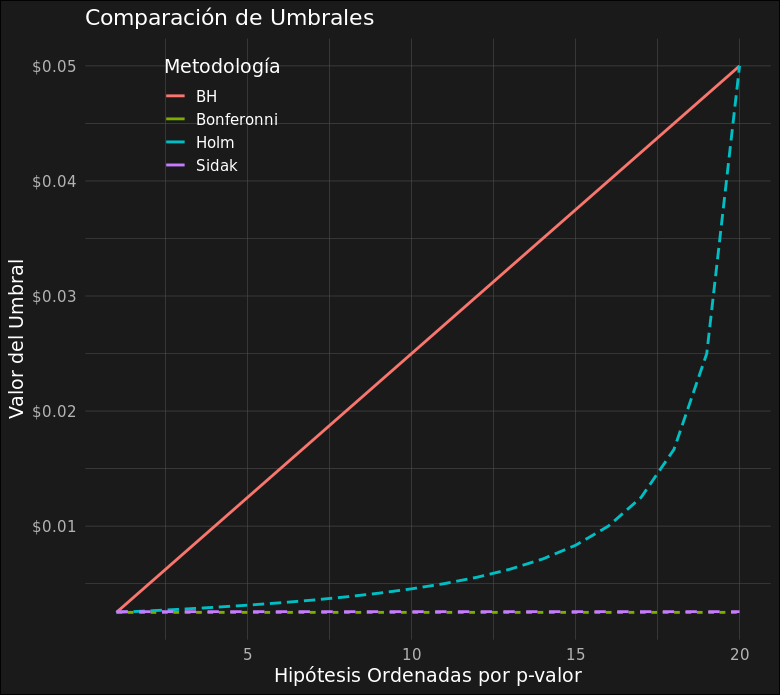
\includegraphics[scale=.39]{comparacion_de_metodos.png}
\caption{Comparación del valor del Umbral de rechazo}
\end{figure}
\end{frame}

\section{MCP - Ciencia de datos.}
\begin{frame}{Aplicación del control FDR en neurociencia}
    
    	\begin{itemize}[<+- | alert@+>]
		
		\item En este ejemplo, se realizó un análisis de las masas en imágenes de resonancia magnética (RM) extraídas de la iniciativa de datos abiertos de la serie de acceso abierto de estudios de imágenes (OASIS). Estos datos contienen imágenes ponderadas en T1 de 416 participantes con y sin demencia de entre 18 y 96 años, lo que permite investigar cómo la edad y las enfermedades relacionadas \textbf{con la edad influyen en la morfología cerebral}.\\
		\item El objetivo del estudio fue determinar que partes del cerebro están relacionadas de su edad.
	\end{itemize}

\end{frame}

\begin{frame}{Metodología}
    
    \begin{itemize}[<+- | alert@+>]
		
		\item Para descargar el conjunto de datos de OASIS, visite $http://www.oasis-brains.org/\#data$ y elija el lanzamiento OASIS-1, que contiene imágenes de resonancia magnética (MR) de 416 participantes de entre 18 y 96 años. El archivo de información del participante incluye variables demográficas básicas (edad, género, mano de obra, nivel educativo, estatus socioeconómico), variables clínicas y estimaciones de volumen cerebral. 
		
		\item[] \begin{figure}[H]
\centering 
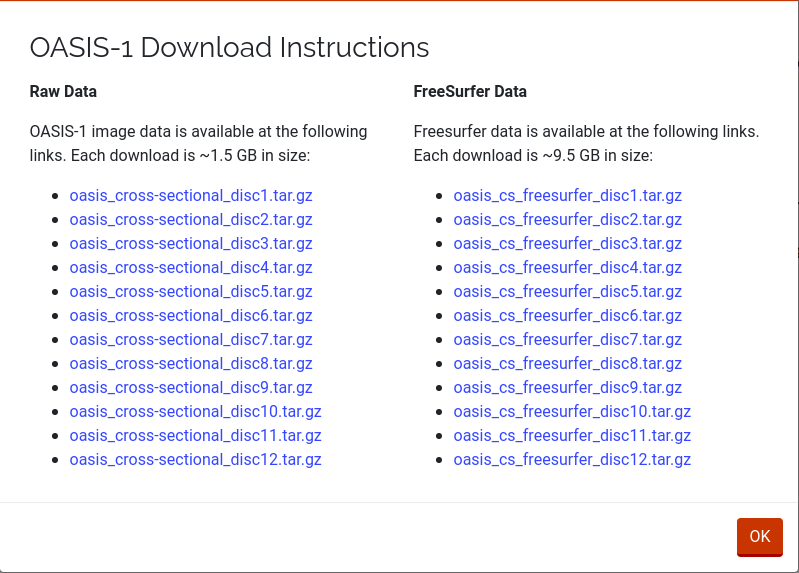
\includegraphics[scale=.19]{descarga_datos.png}
\end{figure}
	\end{itemize}
\end{frame}

\begin{frame}
    Se considero calcular los coeficientes de correlación Spearman  entre el grosor cortical y la edad en cada vóxel cortical, y se consideraron 163810 pruebas de la siguiente forma
\begin{align*}
H_{0i}: \rho_s =0 \ \ \ vs \ \ \ H_{0i}:\rho_s\neq 0, \ \ \forall i=1,\cdots, 163810.
\end{align*}
donde $\rho_s=1-\frac{6\sum d_i^2}{n(n^2-1)}$ y $d_i=rg(X_i)-rg(Y_i)$ es la diferencia de los rangos de cada observación. Se puede probar que si $n$ es grande entonces 
$$\rho_s\sqrt{\frac{n-2}{1-\rho_s^2}} \sim t_{n-2}$$
\end{frame}

\begin{frame}
    \begin{itemize}[<+- | alert@+>]
		
		\item Considerando lo anterior procedió a calcular los p$-$values de cada juego de hipótesis. Y posterior se le aplicaron las correcciones de Sidák para controlar el family$-$wise error rate (FWER), y el procedimiento BH para controlar la FDR. 
		
		\item Un total del $55\%$ de los vóxel mostró un efecto estadísticamente significativo del envejecimiento sobre el grosor cortical usando la corrección de Sidak. Por el contrario, cuando la corrección se basó en el procedimiento Benjamini-Hochberg, el número de vértices significativos fue del $82\%$, lo que sugiere un efecto más generalizado. El nivel crítico sin corregir se fijó en $\alpha = 0.05$ en ambos análisis.
	\end{itemize}
    
\end{frame}

\begin{frame}{Comparación}
Los resultados se muestran en la figura (\ref{cerebro}), lo cuál podemos concluir que algunos de los mayores efectos relacionados con la edad se observan en el surco central.
    \begin{figure}[H]
        \centering \label{cerebro}
        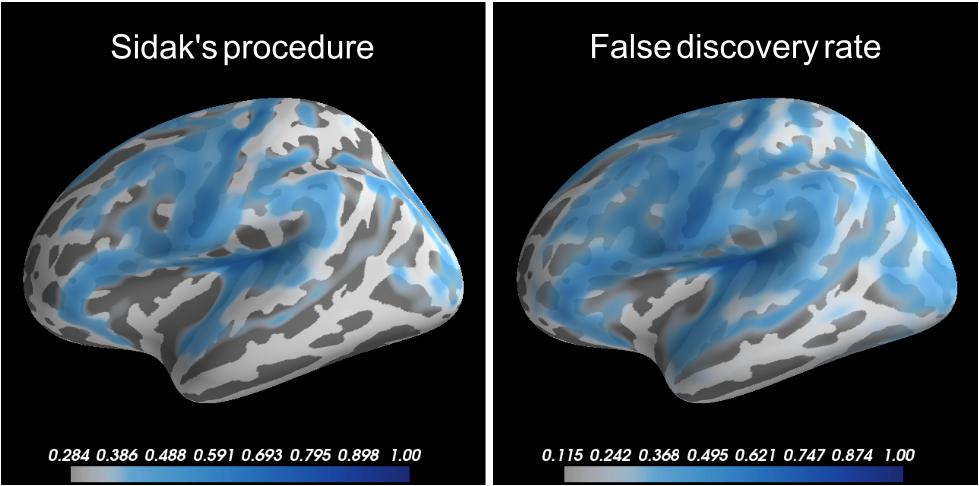
\includegraphics[scale=.29]{neurociencia_FDR_FWER.png}
        \caption{Diferencias cuando se controla el FWER y el FDR.}
    \end{figure}
\end{frame}

\begin{frame}{Artículos interesantes de ejemplos...}
    \begin{itemize}[<+- | alert@+>]
	\item Y. Benjamini and Y. Gavrilov, A Simple Forward Selection Procedure Based On False Discovery Rate Control(2009). 
	
	\item Christopher J. Miller (1) et. al., Controling the False-Discovery Rate in Astrophysical Data Analysis(2001). 
	
	'\textit{El propósito de este artículo es presentar el procedimiento FDR a la comunidad astrofísica. Ilustramos el poder de FDR a través de varios ejemplos astronómicos, incluida la detección de características frente a una función unidimensional suave, por ejemplo, ver las \textit{ondulaciones de bariones} en un espectro de potencia de fluctuaciones de materia y detección de píxeles de origen en datos de imágenes...}'
	\end{itemize}
\end{frame}


\begin{frame}{Conclusiones}
    
    \begin{itemize}[<+- | alert@+>]
	\item Se presentaron las bases teóricas sobre las pruebas de hipótesis múltiples desde el enfoque clásico controlando la $FWER$ y la revolucionaria idea que propusieron Benjamini y Hochberh [1995] sobre controlar la $FDR$.
	
	\item La teórica presentada en este documento como se mencionó son las bases de $MCP$, en la actualidad ya existen una gran variedad de metodologías para controlar $FDR$ y $FWER$ la mayoría es son modificaciones del método de Bonferroní y $BH$.
	\end{itemize}
	
\end{frame}

%------Ejemplos en Ciencia de Datos-----------
\include{ejemplos_DS}



%-----------quitando el siguiente comentario se pueden compilar los ejemplos del archivo ejemplos.tex
%\section{Notación}

\begin{frame}{Ecuaciones}
	
		\begin{equation}\label{Monna}
		\rho: \sum_{j=\gamma}^{\infty} a_{j} p^{j} \mapsto \sum_{j=\gamma}^{\infty} a_{j} p^{-j-1}, \quad a_{j}=0,1, \ldots, p-1, \quad \gamma \in \mathbb{Z}.
		\end{equation}
\end{frame}

\begin{frame}{Transiciones}
	\begin{itemize}[<+- | alert@+>]
		
		\item ítem 1
		\item ítem 2
		\item ítem 3
		
	\end{itemize}

\end{frame}

\subsection{Sección para la tabla}%para que aparezca en la tabla de contenidos como subsección
\section*{Sección} %para que me muestre la barra de progreso

\begin{frame}{Definiciones, teoremas, lemas, corolarios y ejemplos}
	\begin{df}
		La definición.
	\end{df}
\begin{thh}
	El teorema
\end{thh}
\begin{crr}
	El corolario
\end{crr}
\begin{lm}
	El lema
\end{lm}
\begin{example}{Ejemplo}
	El ejemplo
\end{example}
\end{frame}



\begin{frame}[fragile]{Listings en este beamer}
	Sea $x=342.536_7=6\cdot7^{-3}+3\cdot7^{-2}+5\cdot7^{-1}+2\cdot7^0+4\cdot7+3\cdot7^2$

\begin{lstlisting}[language=Python, caption = Instancia de la clase Número   (Number), basicstyle=\tiny]
digits = [3,4,2,5,3,6]
x = Number(7,-3,2,digits) #initialization of x

x.show()
>> [3,4,2,5,3,6]

x.order()
>> -2

x.norm()
>> 49

x.len()
>>6
\end{lstlisting}
En este caso $p=7$, $n=-3$ y  $N=2$. Además satisface que $7^{-3}\leq{x}\leq 7^2$.
\end{frame}


\begin{frame}{Subfiguras}
	
\begin{figure}
	\captionsetup[subfigure]{font=footnotesize}
	\centering
	\subcaptionbox{Triángulo 1}[.5\textwidth]{%
		\begin{tikzpicture}
		
		%   \draw [black!20]  (0,0) grid  (3,4);
		\draw[black]  (0,0)-- (3,0)--  (1.5,4)--cycle;
		
		
		\draw  (0,0) circle  (0pt) node[anchor=north] {$y$};
		\draw  (3,0) circle  (0pt) node[anchor=north] {$z$};
		\draw  (1.5,4.5) circle  (0pt) node[anchor=north] {$x$};
		\draw  (3.5,2) circle  (0pt) node[anchor=north] {${x-z}$};
		\draw  (-0.5,2) circle  (0pt) node[anchor=north] {${x-y}$};
		\draw  (1.5,-0.2) circle  (0pt) node[anchor=north] {${z-y}$};  
		\end{tikzpicture}
	}%
	\subcaptionbox{Triángulo 2}[.5\textwidth]{
		\begin{tikzpicture}
		
		%   \draw [black!20]  (0,0) grid  (3,4);
		\draw[orange]  (0,0)-- (3,0)--  (1.5,4)--cycle;
		
		
		\draw  (0,0) circle  (0pt) node[anchor=north] {$y$};
		\draw  (3,0) circle  (0pt) node[anchor=north] {$z$};
		\draw  (1.5,4.5) circle  (0pt) node[anchor=north] {$x$};
		\draw  (3.5,2) circle  (0pt) node[anchor=north] {${x-z}$};
		\draw  (-0.5,2) circle  (0pt) node[anchor=north] {${x-y}$};
		\draw  (1.5,-0.2) circle  (0pt) node[anchor=north] {${z-y}$};  
		\end{tikzpicture}
	}
\end{figure}
\end{frame}



\section*{Gracias \blacksmiley{}}

\begin{frame}[allowframebreaks]
	\frametitle{Referencias} 
	\begin{thebibliography}{100} % 100 is a random guess of the total number of
		%references
		\bibitem{bib1} Referencia \emph{Javeriana}, 2020.
		
	\end{thebibliography}
\end{frame}


\end{document}